\documentclass[12pt]{report}
\usepackage[utf8]{inputenc}
\usepackage[russian]{babel}
%\usepackage[14pt]{extsizes}
\usepackage{listings}
\usepackage{graphicx}
\usepackage{amsmath,amsfonts,amssymb,amsthm,mathtools} 
\usepackage{pgfplots}
\usepackage{filecontents}
\usepackage{indentfirst}
\usepackage{eucal}
\usepackage{enumitem}
\frenchspacing

\usepackage{indentfirst} % Красная строка


\usetikzlibrary{datavisualization}
\usetikzlibrary{datavisualization.formats.functions}

\usepackage{amsmath}




% Для листинга кода:
\lstset{ %
language=python,                 % выбор языка для подсветки
basicstyle=\small\sffamily, % размер и начертание шрифта для подсветки кода
numbers=left,               % где поставить нумерацию строк (слева\справа)
numberstyle=\tiny,           % размер шрифта для номеров строк
stepnumber=1,                   % размер шага между двумя номерами строк
numbersep=5pt,                % как далеко отстоят номера строк от подсвечиваемого кода
showspaces=false,            % показывать или нет пробелы специальными отступами
showstringspaces=false,      % показывать или нет пробелы в строках
showtabs=false,             % показывать или нет табуляцию в строках
frame=single,              % рисовать рамку вокруг кода
tabsize=2,                 % размер табуляции по умолчанию равен 2 пробелам
captionpos=t,              % позиция заголовка вверху [t] или внизу [b] 
breaklines=true,           % автоматически переносить строки (да\нет)
breakatwhitespace=false, % переносить строки только если есть пробел
escapeinside={\#*}{*)}   % если нужно добавить комментарии в коде
}

\usepackage[left=2cm,right=2cm, top=2cm,bottom=2cm,bindingoffset=0cm]{geometry}
% Для измененных титулов глав:
\usepackage{titlesec, blindtext, color} % подключаем нужные пакеты
\definecolor{gray75}{gray}{0.75} % определяем цвет
\newcommand{\hsp}{\hspace{20pt}} % длина линии в 20pt
% titleformat определяет стиль
\titleformat{\chapter}[hang]{\Huge\bfseries}{\thechapter\hsp\textcolor{gray75}{|}\hsp}{0pt}{\Huge\bfseries}


% plot
\usepackage{pgfplots}
\usepackage{filecontents}
\usetikzlibrary{datavisualization}
\usetikzlibrary{datavisualization.formats.functions}

\begin{document}
\thispagestyle{empty}
\begin{titlepage}
	\noindent \begin{minipage}{0.15\textwidth}
	
\includegraphics[width=\linewidth]{b_logo}
	\end{minipage}
	\noindent\begin{minipage}{0.9\textwidth}\centering
		\textbf{Министерство науки и высшего образования Российской Федерации}\\
		\textbf{Федеральное государственное бюджетное образовательное учреждение высшего образования}\\
		\textbf{~~~«Московский государственный технический университет имени Н.Э.~Баумана}\\
		\textbf{(национальный исследовательский университет)»}\\
		\textbf{(МГТУ им. Н.Э.~Баумана)}
	\end{minipage}
	
	\noindent\rule{18cm}{3pt}
	\newline\newline
	\noindent ФАКУЛЬТЕТ $\underline{\text{«Информатика и системы управления»}}$ \newline\newline
	\noindent КАФЕДРА $\underline{\text{«Программное обеспечение ЭВМ и информационные технологии»}}$\newline\newline\newline\newline\newline
	
	
	\begin{center}
		\noindent\begin{minipage}{1.3\textwidth}\centering
			\Large\textbf{  Отчет по лабораторной работе №4}\newline
			\textbf{по дисциплине "Анализ алгоритмов"}\newline\newline
		\end{minipage}
	\end{center}
	
	\noindent\textbf{Тема} $\underline{\text{Параллельные вычисления применительно к задаче умножения матриц}}$\newline\newline
	\noindent\textbf{Студент} $\underline{\text{Андрич К. }}$\newline\newline
	\noindent\textbf{Группа} $\underline{\text{ИУ7И-56Б}}$\newline\newline
	\noindent\textbf{Оценка (баллы)} $\underline{\text{~~~~~~~~~~~~~~~~~~~~~~~~~~~}}$\newline\newline
	\noindent\textbf{Преподаватели} $\underline{\text{Волкова Л.Л.}}$\newline\newline\newline
	
	\begin{center}
		\vfill
		Москва~---~\the\year
		~г.
	\end{center}
\end{titlepage}


\tableofcontents

\newpage
\chapter*{Введение}
\addcontentsline{toc}{chapter}{Введение}
Термин «матрица» применяется во множестве разных областей: от программирования до кинематографии.

Матрица в математике – это таблица чисел, состоящая из определенного количества строк (m) и столбцов (n).

Мы встречаемся с матрицами каждый день, так как любая числовая информация, занесенная в таблицу, уже в какой-то степени считается матрицей.

Примером могут служить:

\begin{itemize}
	\item список телефонных номеров;
	\item различные статистические данные;
	\item табель успеваемости ученика и многое другое.
\end{itemize}

Целью данной лабораторной работы является изучение возможностей параллельных вычислений приминительно к задаче умножения матриц, в частности, умножения матриц с применением алгоритма Винограда.

В рамках достижения поставленной цели требуется решить следующие задачи: 
\begin{itemize}
	\item изучить алгоритм умножения матриц Винограда;
	\item разработать схемы распараллеливания алгоритма Винограда умножения матриц; 
	\item реализовать алгоритмы умножения матриц линейно и согласно разработанным схемам параллельных вычислений;
	\item экспериментально подтвердить различия во временнóй эффективности линейной и параллельных реализаций на материале замеров времени выполнения реализации на квадратных матрицах переменных размерностей;
	\item описать и обосновать полученные результаты в отчете.
\end{itemize}

\chapter{Аналитическая часть}

В данном разделе будут изучены алгоритмы умножения матрицы и параллельные вычисления.

\section{Определение матрицы и операции умножения матриц}

Матрицей A размера $[N \times M]$ называется прямоугольная таблица чисел, функций или алгебраических выражений, которая представляет собой совокупность $N$ строк и $M$ столбцов, на пересечении которых находятся элементы~\cite{matr}.

Для двух матриц определена операция умножения, если число столбцов в первой матрице совпадает с числом строк во второй.

Пусть даны две прямоугольные матрицы А и В размеров $[N \times M]$ и $[M \times Q]$ соответственно. Результатом произведениея матриц $A$ и $B$ будет матрица $C$ размера $[N \times Q]$, элементы $c_{ij}$ которой могут быть вычислены \cite{matr} по формуле \ref{eq:matrix_mult_formula}.

\begin{equation}
	\label{eq:matrix_mult_formula}
	\forall{i \in \{1,\dotsc,N\}}, \forall{j\in \{1,\dotsc,Q\}}: \\
	c_{i,j} = \sum\limits_{k=1}^M a_{i,k}\cdot b_{k,j}
\end{equation}


\section{Алгоритм умножения матриц Винограда}

Рассмотрим два вектора $V = (v1, v2, v3, v4)$ и $W = (w1, w2, w3, w4)$. 

Их скалярное произведение равно:
\begin{equation}
	\begin{aligned}
		\label{eq:vector_mult_formula}
		V \cdot W=v_1 \cdot w_1 + v_2 \cdot w_2 + v_3 \cdot w_3 + v_4 \cdot w_4
	\end{aligned}
\end{equation}


Это равенство можно переписать в виде \ref{eq:vector_mult_formula_odd}.
\begin{equation}
	\begin{aligned}
		\label{eq:vector_mult_formula_odd}
		V \cdot W=(v_1 + w_2) \cdot (v_2 + w_1) + (v_3 + w_4) \cdot (v_4 + w_3) - v_1 \cdot v_2 -\\
		- v_3 \cdot v_4 - w_1 \cdot w_2 - w_3 \cdot w_4
	\end{aligned}
\end{equation}

Для векторов, размер которых --- нечетное число, равенство \ref{eq:vector_mult_formula_odd} принимает вид \ref{eq:vector_mult_formula_nodd}.  
\begin{equation}
	\label{eq:vector_mult_formula_nodd}
	\begin{aligned}
		V \cdot W=(v_1 + w_2) \cdot (v_2 + w_1) + (v_3 + w_4) \cdot (v_4 + w_3) - v_1 \cdot v_2 -\\
		- v_3 \cdot v_4 - w_1 \cdot w_2 - w_3 \cdot w_4 + v_5 \cdot w_5
	\end{aligned}
\end{equation}

Эти два равенства --- \ref{eq:vector_mult_formula_odd} и \ref{eq:vector_mult_formula_nodd} --- могут быть обобщены на вектора произвольного размера.

Принцип алгоритма Винограда заключается в использовании равенств вида \ref{eq:vector_mult_formula_odd} и \ref{eq:vector_mult_formula_nodd} в рамках умножения матриц --- так, под векторами $V$ и $W$ понимаются строка певрой матрицы и столбец второй матрицы соответственно.

Выражение в правой части равенств \ref{eq:vector_mult_formula_odd} допускает предварительную обработку: его части $(v_1 \cdot v_2 + v_3 \cdot v_4)$ и $(w_1 \cdot w_2 + w_3 \cdot w_4)$ можно вычислить заранее и запомнить для каждой строки первой матрицы и для каждого столбца второй соответсвенно. 

Так, при вычислении $V \cdot W$ с использованием предварительно вычисленных значений нам необходимо выполнить лишь первые два умножения --- $(v_1 + w_2) \cdot (v_2 + w_1)$ и $(v_3 + w_4) \cdot (v_4 + w_3)$ --- и посчитать линейную комбинацию полученных значения согласно формуле \ref{eq:vector_mult_formula_odd}.

В случае умножения матриц, строка и столбец которых преставляют собой вектора нечетного размера, схема рассчета элементов результирующей матрицы сохраняется. После чего, к каждому элементу $c_{ij}$ результирующей матрицы прибавляется число $v_{im} \cdot u_{mj}$, где $v_{im}$ - последний элемент $i$-той строки первой матрицы, $u_{mj}$ - последний элемент $j$-того столбца второй матрицы.

\section{Параллельные вычисления}

При использовании многопроцессорных вычислительных систем с общей памятью обычно предполагается, что имеющиеся в составе системы процессоры обладают равной производительностью, являются равноправными при доступе к общей памяти, и время доступа к памяти является одинаковым (при одновременном доступе нескольких процессоров к одному и тому же элементу памяти очередность и синхронизация доступа обеспечивается на аппаратном уровне).

Распространенный подход при организации вычислений для многопроцессорных вычислительных систем с общей памятью – создание новых параллельных методов на основе обычных последовательных программ. 

Для реализации алгоритма на параллельной системе его следует представить в виде последовательности групп операций, причем операции в каждой группе могут быть выполнены одновременно - то есть каждая операция любой группы зависит либо от входных данных, либо от результатов выполнения операций в предыдущих группах, но не зависит от результатов выполнения других операций в той же группе.

Одновременное выполнение операций группы параллельной системой поддерживается на уровне операционной системы с помощью механизма потоков.  

Потоки исполняются в общем адресном пространстве параллельной программы. Как результат, взаимодействие параллельных потоков можно организовать через использование общих данных, являющихся доступными для всех потоков. Наиболее простая ситуация состоит в использовании общих данных только для чтения. В случае же, когда общие данные могут изменяться несколькими потоками, необходимы специальные усилия для организации правильного взаимодействия --- очередного обращения к данным для записи.

\section{Вывод}
	В данном разделе были описаны цели и задачи лабораторной работы, изучены алгоритмы умножения матрицы и параллельные вычисления.
	
\clearpage

\chapter{Конструкторская часть}

\section{Схемы алгоритмов}
На рисунках \ref{fig:p1}, \ref{fig:p2}, \ref{fig:p3} и \ref{fig:p4} приведена схема алгоритма умножения матриц Винограда.

\begin{figure}[h]
	\centering
	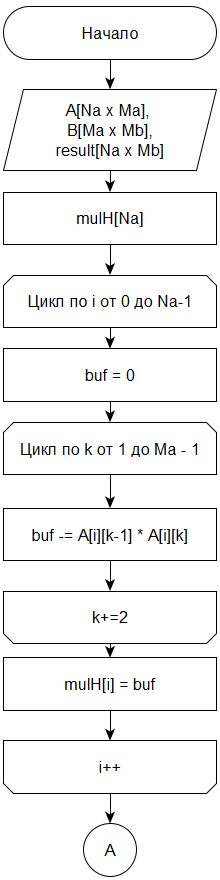
\includegraphics[width=0.21\linewidth]{p1.png}
	\caption{Схема алгоритма Винограда умножения матриц, часть 1}
	\label{fig:p1}
\end{figure}

\newpage

\begin{figure}[h]
	\centering
	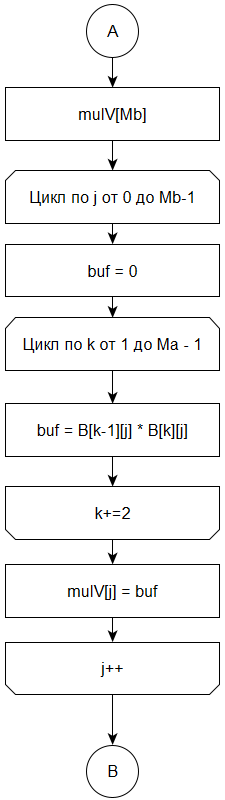
\includegraphics[scale=1]{p2.png}
	\caption{Схема алгоритма Винограда умножения матриц, часть 2}
	\label{fig:p2}
\end{figure}

\newpage

\begin{figure}[h]
	\centering
	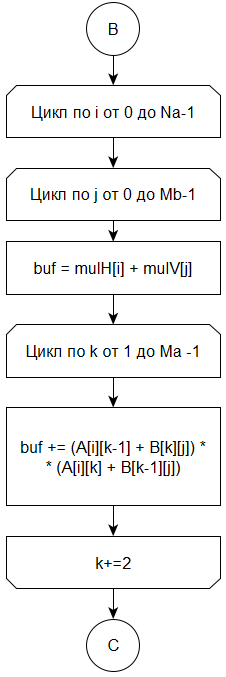
\includegraphics[scale=1.1]{p3.png}
	\caption{Схема алгоритма Винограда умножения матриц, часть 3}
	\label{fig:p3}
\end{figure}

\newpage

\begin{figure}[h]
	\centering
	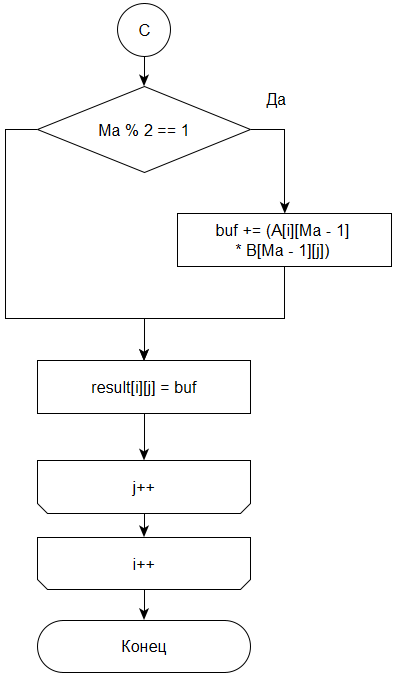
\includegraphics[scale=1.1]{p4.png}
	\caption{Схема алгоритма Винограда умножения матриц, часть 4}
	\label{fig:p4}
\end{figure}

\newpage

\section{Распараллеливание задачи}

\begin{enumerate}
	\item 
	Рассмотрим первые два цикла алгоритма, вычисление произведений пар последовательных элементов каждой строки первой матрицы и каждого столбца второй. Вычисления произведений для каждой из строк первой матрицы не зависят от результатов вычислений для других строк. Вычисления произведений для каждого столбца второй матрицы не зависят от результатов вычислений для других столбцов. Вместе с тем, вычисления для строк первой матрицы не зависят от результатов вычислений для столбцов второй. Участок алгоритма, содержащий два первых цикла, может быть распараллелен по подмножествам строк первой матрицы и по подмножествам столбцов второй: каждый поток будет выполнять предварительные вычисления для определенного подмножества строк первой матрицы или для определенного подмножества столбцов второй. Рассмотрим этот подход в качестве первой схемы параллельных вычислений.
	
	\item 
	
	Рассмотрим участок алгоритма с заполнением результирущей матрицы: вычисление элемента результирующей матрицы для каждой строки первой матрицы не зависит от результатов вычислений для других строк. Можно распараллелить участок алгоритма с заполнением результирующей матрицы по подмножествам строк: каждый поток будет выполнять вычисления для определенного подмножетсва строк результирующей матрицы. В этом участке находятся три вложенных цикла --- именно этот участок алгоритма имеет наибольшую сложность. Рассмотрим этот подход в качестве второй схемы параллельных вычислений. 
\end{enumerate}

Таким образом, для изучения выбрано две схемы параллельных вычислений:
\begin{itemize}
	\item распараллеливание участка алгоритма, содержащего первые два цикла с предварительными вычислениями произведений пар элементов для каждой строки первой матрицы и каждого столбца второй по подмножествам строк первой матрицы и подмножествам столбцов второй;
	\item распараллеливание участка алгоритма, содержащего три вложенных цикла с вычислением элементов результирующей матрицы по подмножествам строк результирующей матрицы.
\end{itemize}

Предположительно, из двух описанных схем наибольшую выгоду принесет вторая --- распараллеливание участка алгоритма, который содержит три вложенных цикла. Это предположение будет в дальнейшем проверено в исследовательском разделе.

\section{Вывод}
	Была описана структура программного комплекса и схемы алгоритмов, так же проведены функциональные тесты работы программы, сделано предположение о том, какая из схем параллельных вычислений окажется эффективнее.

\chapter{Технологическая часть}

В этом разделе будет обоснован выбор языка програмирования, описаны технические характеристики,приведены листинги кода реализованных алгоритмов.

\section{Выбор ЯП}
В качестве языка программирования мной был выбран С++ так как этот язык удобен для работы с потоками.
Для замера времени выполнения использовалась функция $high\_resolution\_clock::now()$.

\section{Требование к ПО}

\begin{itemize}
	\item корректное умножение двух матриц;
	\item при матрицах неправилыных размеров программа не должна аварийно завершаться.
\end{itemize}

\section{Реализация алгоритмов}

В следующем разделе представлены листинги реализаций алгоритма Винограда.
В листинге \ref{lst:lin} представлена линейная реализация алгоритма умножения матриц Винограда. В листингах \ref{lst:par_1} и \ref{lst:par_2} представлены реализации алгоритма согласно разработанным схемам параллельных вычислений.

\newpage

\begin{lstlisting}[label={lst:lin},caption=Линейная реализация алгоритма Винограда умножения матриц]
	int vng_mult(int** A, int** B, int** result, int N_a, int M_a, int M_b)
	{
		int* mulH = new int[N_a];
		int* mulV = new int[M_b];
		
		// PART 1
		int buf;
		for (int i = 0; i < N_a; i++)
		{
			buf = 0;
			for (int k = 1; k < M_a; k += 2)
			buf -= A[i][k - 1] * A[i][k];
			mulH[i] = buf;
		}
		
		// PART 2
		for (int j = 0; j < M_b; j++)
		{
			buf = 0;
			for (int k = 1; k < M_a; k += 2)
			buf -= B[k - 1][j] * B[k][j];
			mulV[j] = buf;
		}
		
		// PART 3 + 4
		for (int i = 0; i < N_a; i++)
		for (int j = 0; j < M_b; j++)
		{
			buf = mulH[i] + mulV[j];
			for (int k = 1; k < M_a; k += 2)
			buf += (A[i][k - 1] + B[k][j]) * (A[i][k] + B[k - 1][j]);
			
			if (M_a % 2)
			buf += A[i][M_a - 1] * B[M_a - 1][j];
			
			result[i][j] = buf;
		}
		
		return SUCCESS;
	}
	
\end{lstlisting}

\newpage

\begin{lstlisting}[label={lst:par_1},caption=caption=Реализация алгоритма Винограда умножения матриц с использованием первой схемы параллельных вычислений]
	int vng_mult_par1(int** A, int** B, int** result, int N_a, int M_a, int M_b)
	{
		int* mulH = new int[N_a];
		int* mulV = new int[M_b];
		std::thread* threads = new std::thread[t_count];
		
		if (t_count > 1)
		{
			int proportion = t_count * N_a / (N_a + M_b);
			int rows_t = (proportion) ? proportion : 1;
			int cols_t = t_count - rows_t;
			
			int rows_per_t = N_a / rows_t;
			int cols_per_t = M_b / cols_t;
			
			int start_row = 0;
			for (int i = 0; i < rows_t; i++)
			{
				int end_row = (i == rows_t - 1) ? N_a : start_row + rows_per_t;
				threads[i] = std::thread(scheme1_part1, A, N_a, M_a, mulH, start_row, end_row);
				start_row = end_row;
			}
			
			int start_col = 0;
			for (int i = rows_t; i < t_count; i++)
			{
				int end_col = (i == t_count - 1) ? M_b : start_col + cols_per_t;
				threads[i] = std::thread(scheme1_part2, B, M_a, M_b, mulV, start_col, end_col);
				start_col = end_col;
			}
			
			for (int i = 0; i < t_count; i++)
			{
				threads[i].join();
			}
		}
	
\end{lstlisting}

\newpage

\begin{lstlisting}
else
{
	int buf;
	for (int i = 0; i < N_a; i++)
	{
		buf = 0;
		for (int k = 1; k < M_a; k += 2)
		buf -= A[i][k - 1] * A[i][k];
		mulH[i] = buf;
	}
	
	for (int j = 0; j < M_b; j++)
	{
		buf = 0;
		for (int k = 1; k < M_a; k += 2)
		buf -= B[k - 1][j] * B[k][j];
		mulV[j] = buf;
	}
}

for (int i = 0; i < N_a; i++)
for (int j = 0; j < M_b; j++)
{
	buf = mulH[i] + mulV[j];
	for (int k = 1; k < M_a; k += 2)
	buf += (A[i][k - 1] + B[k][j]) * (A[i][k] + B[k - 1][j]);
	
	if (M_a % 2)
	buf += A[i][M_a - 1] * B[M_a - 1][j];
	
	result[i][j] = buf;
}

return SUCCESS;
}
}
\end{lstlisting}

\newpage

\begin{lstlisting}
void scheme1_part1(int** A, int N_a, int M_a, int* mulH, int start, int end)
{
	int buf;
	for (int i = start; i < end; i++)
	{
		buf = 0;
		for (int k = 1; k < M_a; k += 2)
		buf -= A[i][k - 1] * A[i][k];
		mulH[i] = buf;
	}
}

void scheme1_part2(int** B, int M_a, int M_b, int* mulV, int start, int end)
{
	int buf;
	for (int j = start; j < end; j++)
	{
		buf = 0;
		for (int k = 1; k < M_a; k += 2)
		buf -= B[k - 1][j] * B[k][j];
		mulV[j] = buf;
	}
\end{lstlisting}

\newpage

\begin{lstlisting}[label={lst:par_2},caption=Реализация алгоритма Винограда умножения матриц с использованием второй схемы параллельных вычислений]
	int vng_mult_par2(int** A, int** B, int** result, int N_a, int M_a, int M_b, int t_count)
	{
		int* mulH = new int[N_a];
		int* mulV = new int[M_b];
		std::thread* threads = new std::thread[t_count];
		
		int buf;
		for (int i = 0; i < N_a; i++)
		{
			buf = 0;
			for (int k = 1; k < M_a; k += 2)
			buf -= A[i][k - 1] * A[i][k];
			mulH[i] = buf;
		}
		
		for (int j = 0; j < M_b; j++)
		{
			buf = 0;
			for (int k = 1; k < M_a; k += 2)
			buf -= B[k - 1][j] * B[k][j];
			mulV[j] = buf;
		}
		
		int rows_per_t = N_a / t_count; 
		int start_row = 0;
		for (int i = 0; i < t_count; i++)
		{
			int end_row = (i == t_count - 1) ? N_a : start_row + rows_per_t; 
			threads[i] = std::thread(scheme_2, A, B, result, N_a, M_a, M_b, mulH, mulV, start_row, end_row);
			start_row = end_row;
		}
		
		for (int i = 0; i < t_count; i++)
		{
			threads[i].join();
		}
		
		return SUCCESS;
	}
	
\end{lstlisting}

\newpage

\begin{lstlisting}
void scheme_2(int** A, int** B, int** result, int N_a, int M_a, int M_b, int* mulH, int* mulV, int start_row, int end_row)
{
	int buf;
	for (int i = 0; i < N_a; i++)
	for (int j = 0; j < M_b; j++)
	{
		buf = mulH[i] + mulV[j];
		for (int k = 1; k < M_a; k += 2)
		buf += (A[i][k - 1] + B[k][j]) * (A[i][k] + B[k - 1][j]);
		
		if (M_a % 2)
		buf += A[i][M_a - 1] * B[M_a - 1][j];
		
		result[i][j] = buf;
	}
}
\end{lstlisting}

\section{Тестовые данные}

Результаты тестирования программы приведены в таблице \ref{tab:tests}. В случае, если умножение матриц не допускается при проверке размеров, выводится соответствующее сообщение.

\begin{table}[h]
	\caption{\label{tab:tests}Тесты для проверки корректности программы.}
	\begin{center}
		\begin{tabular}{ | c | c | c | c |}
			\hline
			\textbf{Матрица 1} & \textbf{Матрица 2} & \textbf{Ожидаемый рез.} & \textbf{Фактический рез.}\\ \hline
			$\begin{bmatrix} 
				1&2&3 \\
				2&3&4 \\ 
				3&4&5 \\ 
			\end{bmatrix}$ & 
			$\begin{bmatrix} 
				2&3&4 \\
				3&4&5 \\ 
				4&5&6 \\ 
			\end{bmatrix}$ &
			$\begin{bmatrix} 
				20&26&32 \\
				29&38&47 \\ 
				38&50&67 \\ 
			\end{bmatrix}$ &
			$\begin{bmatrix} 
				20&26&32 \\
				29&38&47 \\ 
				38&50&67 \\ 
			\end{bmatrix} $\\
			\hline
			
			$\begin{bmatrix} 
				1&2&3 \\
				4&5&6 \\ 
				7&8&9 \\ 
			\end{bmatrix}$ & 
			$\begin{bmatrix} 
				1&1&1 \\
				1&1&1 \\ 
			\end{bmatrix}$ &
			$\begin{matrix} 
				\text{Can't multiply matricies} \\
				\text{with such sizes} \\ 
			\end{matrix}$ &
			$\begin{matrix} 
				\text{Can't multiply matricies} \\
				\text{with such sizes} \\ 
			\end{matrix}$\\
			\hline
			
			$\begin{bmatrix} 
				1&2 \\
				2&4 \\ 
				4&8 \\ 
			\end{bmatrix}$ & 
			$\begin{bmatrix} 
				1&2&3 \\
				4&5&6 \\ 
			\end{bmatrix}$ &
			$\begin{bmatrix} 
				9&12&15 \\
				18&24&30 \\ 
				39&48&60 \\ 
			\end{bmatrix}$ &
			$\begin{bmatrix} 
				9&12&15 \\
				18&24&30 \\ 
				39&48&60 \\
			\end{bmatrix}$\\
			\hline
		\end{tabular}
		
	\end{center}
\end{table} 

\section{Вывод}
В данном разделе  был обоснован выбор языка програмирования и приведены листинги кода реализованных алгоритмов.

\chapter{Исследовательская часть}

В данном разделе будут приведены демонстрация работы программы и исследование процессорного времени реализаций алгоритмов.

\section{Пример работы}

Демонстрация работы программы приведена на рисунке 4.1.

\begin{figure}[h]
	\begin{center}
	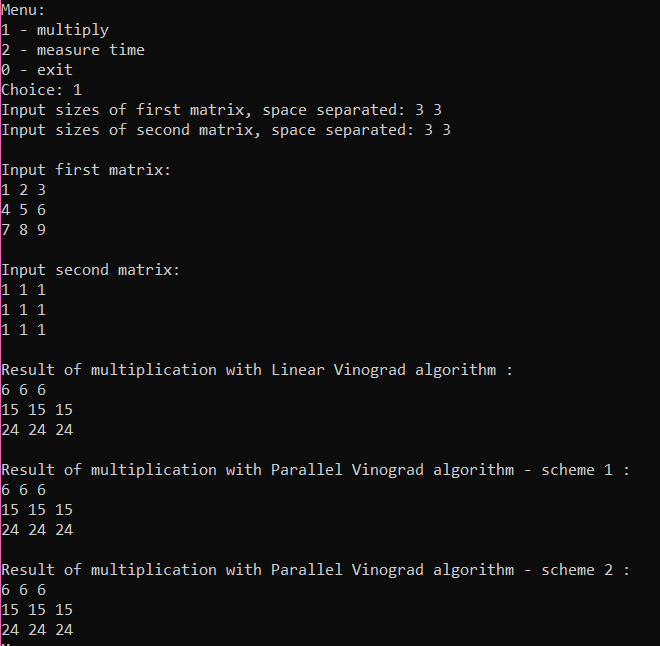
\includegraphics[scale=1]{example.png}
	 \caption{Демонстрация работы программы}
	\end{center}
\end{figure}

\section{Время выполнения алгоритмов}
В следующем разделе приведены результаты замеров времени выполнения реализаций на произвольно заполненных квадратных матрицах. Замеры времени произведены с помощью функции $high\_resolution\_clock::now()$.

Было произведено две серии замеров: 
\begin{itemize}
	\item для матриц размером $N \times N = 500$ при переменном числе потоков для параллельных реализаций;
	\item для матриц размером $N \times N$, $N \in \{ 100, 200, 300, 400, 500 \}$ с постоянным числом потоков для параллельных реализаций, равным 8.
\end{itemize}

Каждый замер времени был произведен на $100$ итерациях, в качетсве результата взято время работы алгоритма, усредненное по всем итерациям.  
\newline

Результаты замеров времени приведены в таблицах \ref{tab:timeanalysis1} и \ref{tab:timeanalysis2}.

\begin{table} [h!]
	\caption{\label{tab:timeanalysis1} Результаты первой серии замеров процессорного времени в мсек. для реализаций алгоритмов умножения матриц}
	\begin{center}
		\begin{tabular}{|c | c | c | c|} 
		 	\hline
			$N$ & Линейно & Паралл. схема 1 & Паралл. схема 2 \\ 
			\hline  
			1 & 429 & 436 & 436 \\
			\hline
			2 & 435 & 331 & 256 \\
			\hline
			4 & 432 & 291 & 211 \\
			\hline
			8 & 422 & 269 & 206 \\
			\hline
			16 & 439 & 157 & 82 \\
			\hline
			32 & 433 & 228 & 102 \\
			\hline
		\end{tabular}
	\end{center}
\end{table}

\begin{figure}[h!]
	\begin{center}
		\begin{tikzpicture}
			\begin{axis}[
				legend pos = north west,
				xlabel=количество потоков в параллельных реализациях,
				ylabel=длина время выпольнения - мсек,
				minor tick num = 1,
				grid = both,
				major grid style = {lightgray},
				minor grid style = {lightgray!25},
				xtick distance = 50,
				width = 0.9\textwidth,
				height = 0.5\textwidth]
				
				\addplot[
				blue,
				semithick,
				mark = x,
				mark size = 3pt,
				thick,
				] file {linear1.txt};
				
				\addplot[
				red,
				semithick,
				mark = x,
				mark size = 3pt,
				thick,
				] file {scheme1.txt};
				
				\addplot[
				green,
				semithick,
				mark = x,
				mark size = 3pt,
				thick,
				] file {scheme2.txt};
				
				\legend{
					Линейна реализация,
					Параллельная схема 1,
					Параллельная схема 2,
				}
			\end{axis}
		\end{tikzpicture}
	\end{center}
	\caption{Результаты первой серии замеров процессорного времени в мсек. для реализаций алгоритмов умножения матриц}
\end{figure}

\newpage

\begin{table} [h!]
	\caption{\label{tab:timeanalysis2} Результаты второй серии замеров процессорного времени в мсек. для реализаций алгоритмов умножения матриц}
	\begin{center}
		\begin{tabular}{|c | c | c | c|} 
			\hline
			$N$ & Линейно & Паралл. схема 1 & Паралл. схема 2 \\ 
			\hline  
			100 & 5 & 26 & 32 \\
			\hline  
			200 & 45 & 132 & 122 \\
			\hline  
			300 & 152 & 166 & 158 \\
			\hline  
			400 & 323 & 232 & 178 \\
			\hline  
			500 & 437 & 269 & 207 \\
			\hline
		\end{tabular}
	\end{center}
\end{table}

\begin{figure}[h!]
	\begin{center}
		\begin{tikzpicture}
			\begin{axis}[
				legend pos = north west,
				xlabel=количество строк квадратной матрицы,
				ylabel=длина время выпольнения - мсек,
				minor tick num = 1,
				grid = both,
				major grid style = {lightgray},
				minor grid style = {lightgray!25},
				xtick distance = 50,
				width = 0.9\textwidth,
				height = 0.5\textwidth]
				
				\addplot[
				blue,
				semithick,
				mark = x,
				mark size = 3pt,
				thick,
				] file {linear2.txt};
				
				\addplot[
				red,
				semithick,
				mark = x,
				mark size = 3pt,
				thick,
				] file {scheme12.txt};
				
				\addplot[
				green,
				semithick,
				mark = x,
				mark size = 3pt,
				thick,
				] file {scheme22.txt};
				
				\legend{
					Линейна реализация,
					Параллельная схема 1,
					Параллельная схема 2,
				}
			\end{axis}
		\end{tikzpicture}
	\end{center}
	\caption{Результаты второй серии замеров процессорного времени в мсек. для реализаций алгоритмов умножения матриц}
\end{figure}

\newpage

Результаты проведенного эксперимента отвечают ожиданиям. 

На входных матрицах небольших размерностей линейная реализация алгоритма работает быстрее, так как имеются накладные расходы на параллельные реализации:
\begin{itemize}
	\item создание потоков;
	\item дополнительные вычисления;
\end{itemize}

Они превышают выгоду во времени на, непосредственно, умножение матриц. При увеличении размерностей входных матриц, выгода во времени на умножение параллельных реализаций превышает накладные расходы, и параллельные реализации выигрывают по времени над линейной. Это продемонстрировано на рисунке 4.3. 

Причем, при увеличении размерностей входных данных, выгода по времени второй схемы параллельных вычислений превышает выгоду первой. На моем устройстве вторая схема параллельных вычислений работает в среднем в $1.3$ раза быстрее, чем первая на таких же вхожных данных, и в $2$ раза быстрее, чем линейная реализация. Это продемонстрировано на рисунке 4.3. 

До определенного момента при увеличении числа потоков время исполнения параллельных реализаций уменьшается на таких же входных данных, но по достижению количества потоков, равного $16$ ( количество логических процессоров устройства, умноженное на 4)снова начинает расти. Это продемонстрировано на рисунке 4.2.

\newpage

\section{Вывод}

В данном разделе были приведены демонстрация работы программы и исследование процессорного времени реализаций алгоритмов, исходя из исследований сделаны выводы об эффективности выбранных схем распарраллеливания данной задачи.


\chapter*{Заключение}
\addcontentsline{toc}{chapter}{Заключение}

В ходе выполнения работы решены следующие задачи:
\begin{itemize}
	\item изучен алгоритм умножения матриц Винограда;
	\item разработаны схемы распараллеливания алгоритма Винограда умножения матриц; 
	\item реализованы алгоритмы умножения матриц --- линейно и согласно разработанным схемам параллельных вычислений;
	\item экспериментально подтверждены различия во временнóй эффективности линейной и параллельных реализаций на материале замеров времени выполнения реализаций на квадратных матрицах;
	\item описаны и обоснованы полученные результаты в отчете.
\end{itemize}

Различия во временной эффективности, подтвержденные экспериментально на материале замеров времени исполнения реализаций, отвечают ожиданиям. 

На входных матрицах небольших размерностей линейная реализация алгоритма работает быстрее, так как накладные расходы на параллельные реализации превышают выгоду во времени. При увеличении размерностей входных матриц, выгода во времени на умножение параллельных реализаций превышает накладные расходы, и параллельные реализации выигрывают по времени над линейной.

При увеличении размерностей входных данных, выгода по времени второй схемы параллельных вычислений превышает выгоду первой. 

Вторая схема параллельных вычислений работает в среднем в $1.3$ раза быстрее, чем первая на таких же вхожных данных, и в $2$ раза быстрее, чем линейная реализация.

Для числа потоков, меньшего $16$ с увеличением числа потоков время исполнения параллельных реализаций уменьшаяется, однако по достижению 16 снова начинает увеличиваться.

\addcontentsline{toc}{chapter}{Список литератури}

\bibliographystyle{utf8gost705u}  % стилевой файл для оформления по ГОСТу

\bibliography{51-biblio}          % имя библиографической базы (bib-файла)

\begin{thebibliography}{9}
		
		\bibitem{Demianov}
		Демьянович Юрий Казимирович О параллельных вычислениях // КИО. 2007. №3. [Электронный ресурс.] URL: https://cyberleninka.ru/article/n/o-parallelnyh-vychisleniyah (дата обращения: 20.10.2021).
		
		\bibitem{Gladyshev}
		Гладышев Е.И., Мурыгин А.В. Многопоточность в приложениях // Актуальные проблемы авиации и космонавтики. 2012. №8. [Электронный ресурс.] URL: https://cyberleninka.ru/article/n/mnogopotochnost-v-prilozheniyah (дата обращения: 20.10.2021).
		
		\bibitem{Zheludkov}
		Антон Владимирович Желудков, Дмитрий Васильевич Макаров, Павел Владимирович Фадеев Исследование программных потоков на примере задачи умножения матриц // Символ науки. 2016. №11-3. [Электронный ресурс.] URL: https://cyberleninka.ru/article/n/issledovanie-programmnyh-potokov-na-primere-zadachi-umnozheniya-matrits (дата обращения: 20.10.2021).
		
		\bibitem{matr}  Умножение матриц.[Электронный ресурс].Режим доступа: https://life-prog.ru/2\_90314\_umnozhenie-matrits.html (дата обращения: 20.10.2021)
\end{thebibliography}

\end{document}
